\section{The Method to Solve the Optimal Problem}
\label{sec_solve_optimal}
In this section, we apply the Algorithm 1 to solve Equation~\ref{equ_final}.
Our algorithm is based on Greedy Algorithm~\cite{Greedy_Algorithm}.
We suppose the input of this algorithm is the graph of the target area $a$ and the set of cost $C_{set}$ consists $c_i, i \in Po^{'}(a)$,
and the graph of the target area $a$ can be generated by the first layer after it processed the original map of target area.
The output of this algorithm is the decision vector that can determine the set of nodes that should be used as the site to construct charging stations.
Algorithm~\ref{alg_solve_optimal} summaries the process of our algorithm.
\begin{algorithm}
\label{alg_solve_optimal}
\small
\caption{{\tt Find\_Optimal\_Solution}($G^{'}_{a}(Po^{'}(a),\theta^{'}(a))$, $C_{set}$)}
\KwIn{$G^{'}_{a}(Po^{'}(a),\theta^{'}(a))$: the graph of target area $a$, \\
$C_{set}$ is the set of cost, $c_i \in C_{set}$ represents the cost of constructing a charging station in site $i$.}
\KwOut{$X$: the vector, $x_i$ is defined in Equation~\ref{equ_decision_x_i}.}
Initialize the vector $X$: Set the length of $X$ equals to the number of elements in $Po_(a)$, the default value of $x_i, i \in Po^{'}_{a}$ is $1$\;
Construct a temporary node set $N_{temp}$of nodes $i$ with $x_i = 1$,
where the induce subgraph is still connected when $x_i$ is set to 0\;
\While{$N_{temp} == \text{NULL}$}{
    $X^{'} \leftarrow X$\;
    $flag \leftarrow 0$\;
    \While{$flag == 0 $ OR $N_{temp} == \text{NULL}$}{
        Select $j$ with the largest $c_i, i \in N_{temp}$\;
        Change $X^{'}$ with $x^{'}_j \leftarrow 0$\;
        \eIf{$X^{'}$ meets $\sum_{j \in Set^{\alpha{R}(i)}} Cap(j) \times x_j \geqslant Demand(i)$}{
                        $X \leftarrow X^{'}$\;
                        $flag \leftarrow 1$\;
                }
                {
                        $x^{'}_j \leftarrow 1$\;
                        Delete $j$ in $N_{temp}$\;
                }
    }
}
\Return {$X$}\;
\end{algorithm}
\begin{figure}[h]
\centering
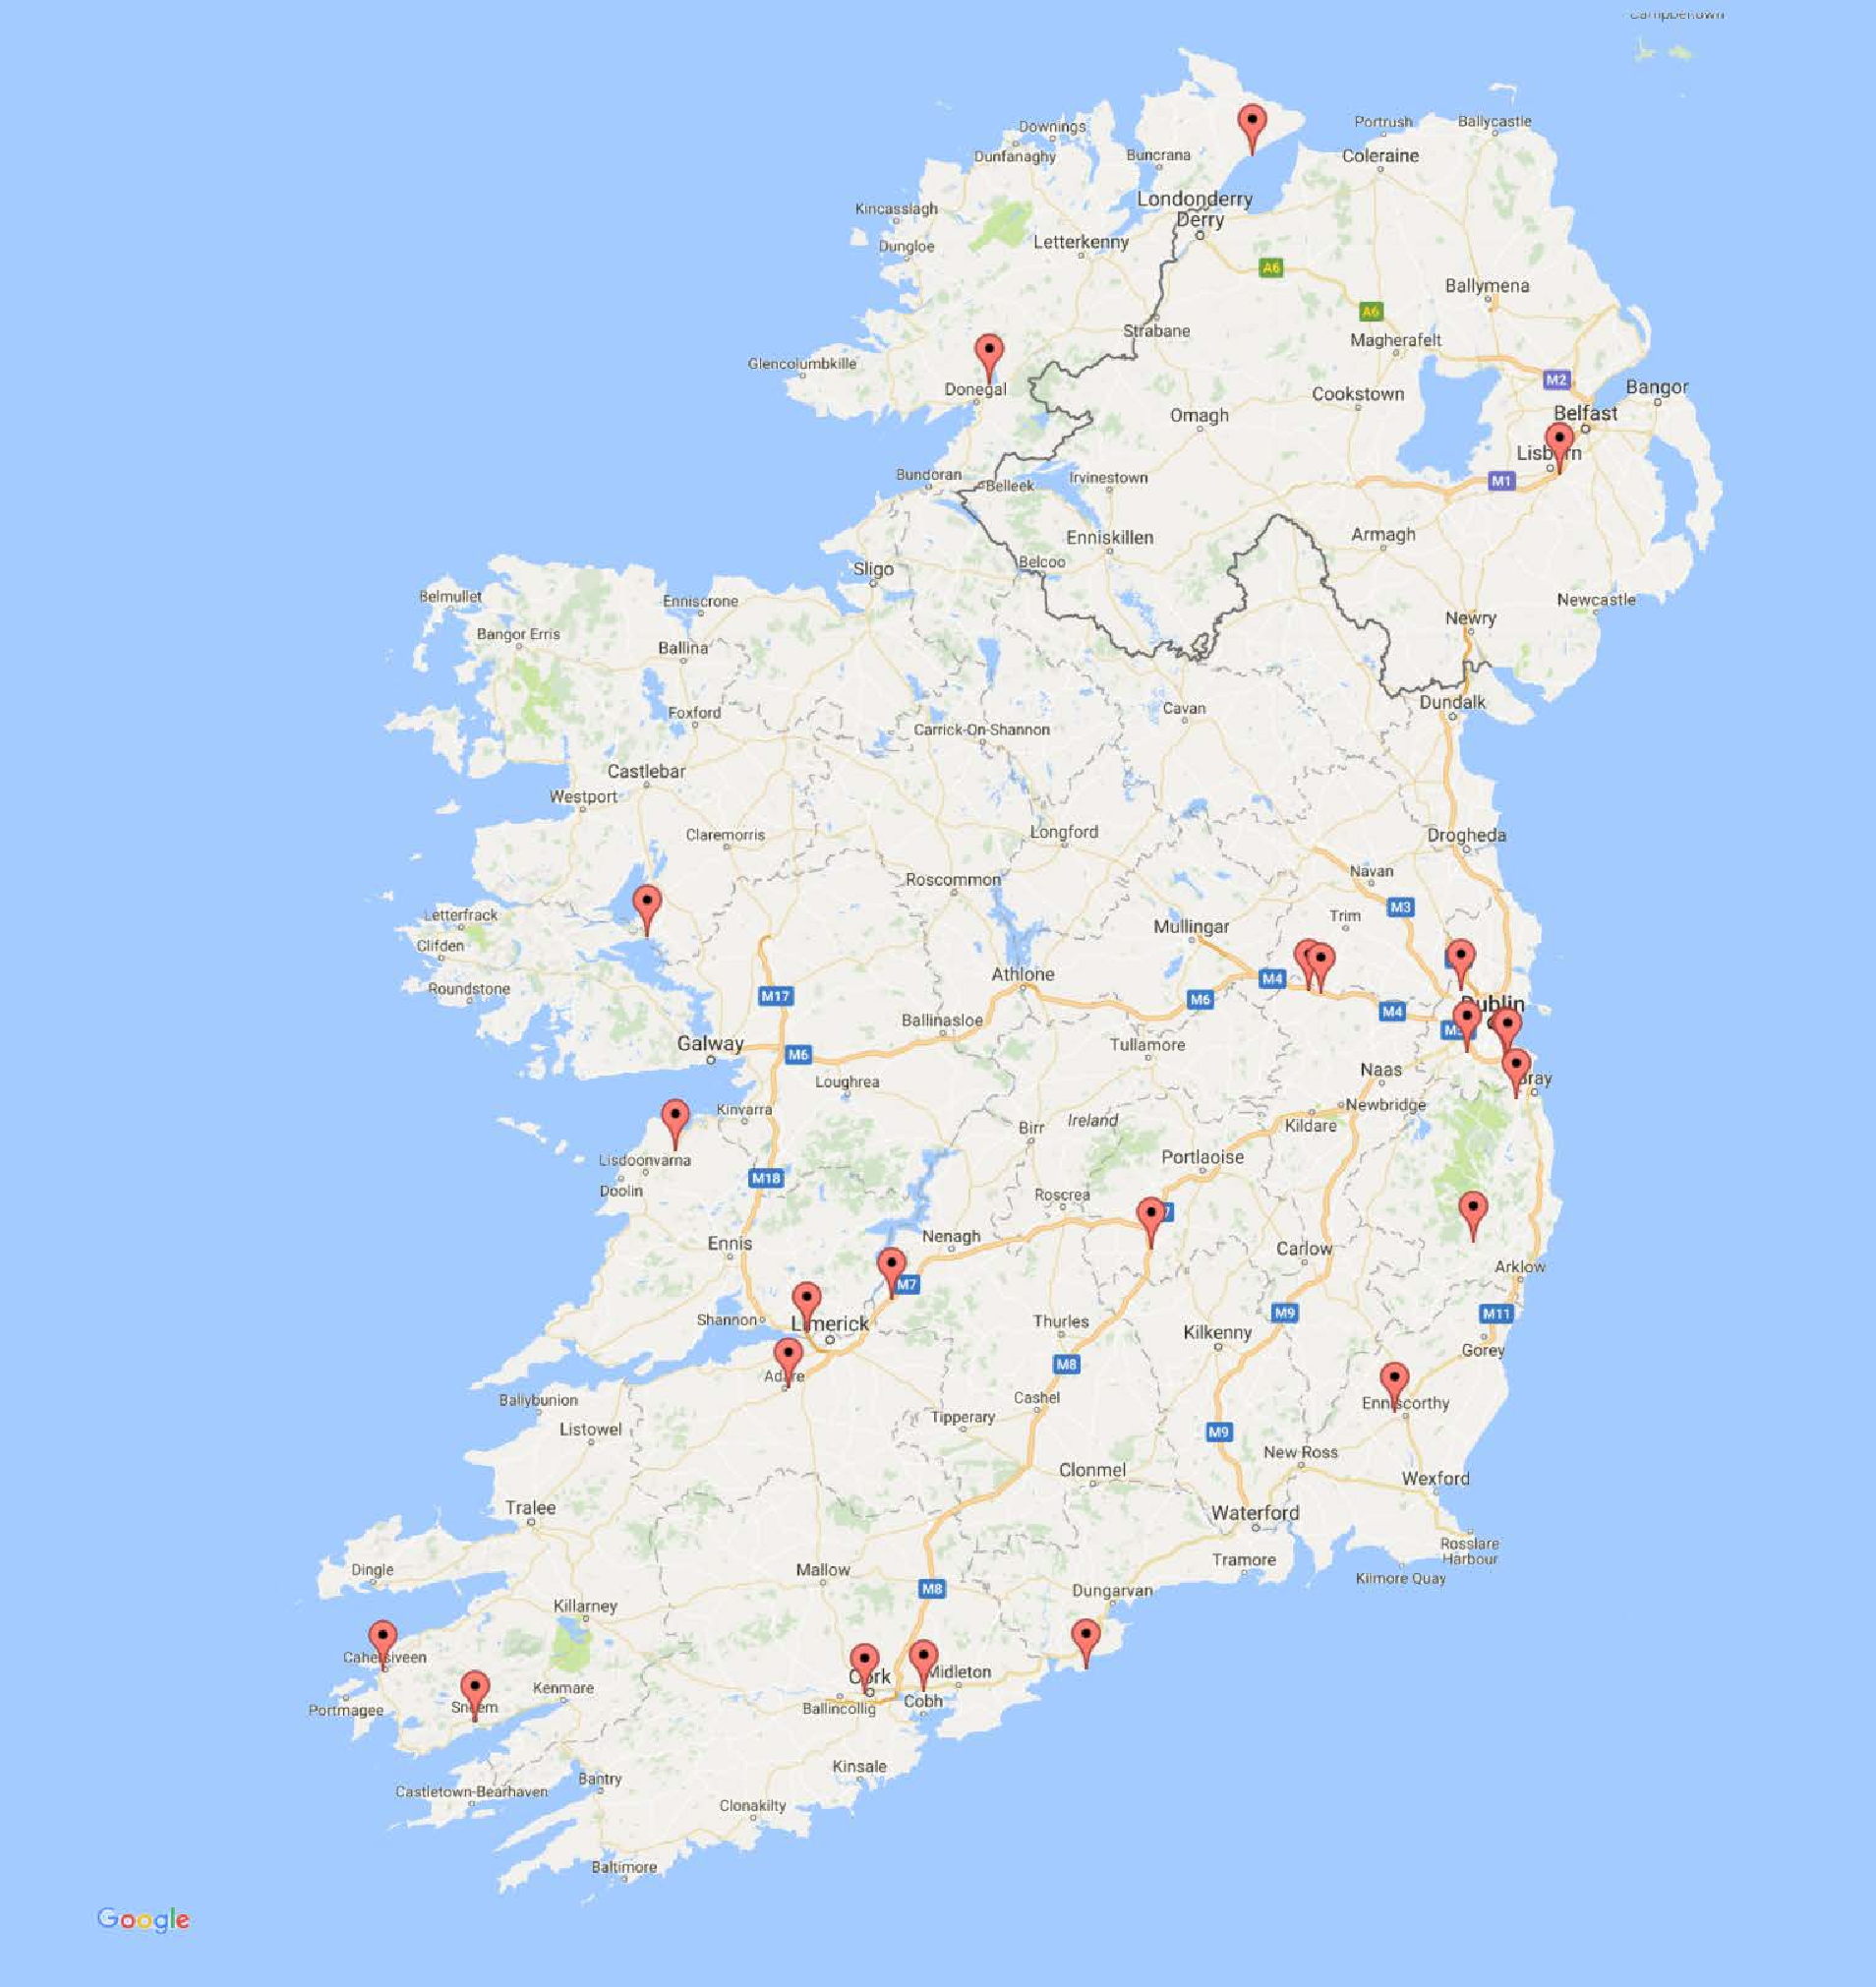
\includegraphics[width=2in]{stage0.pdf}
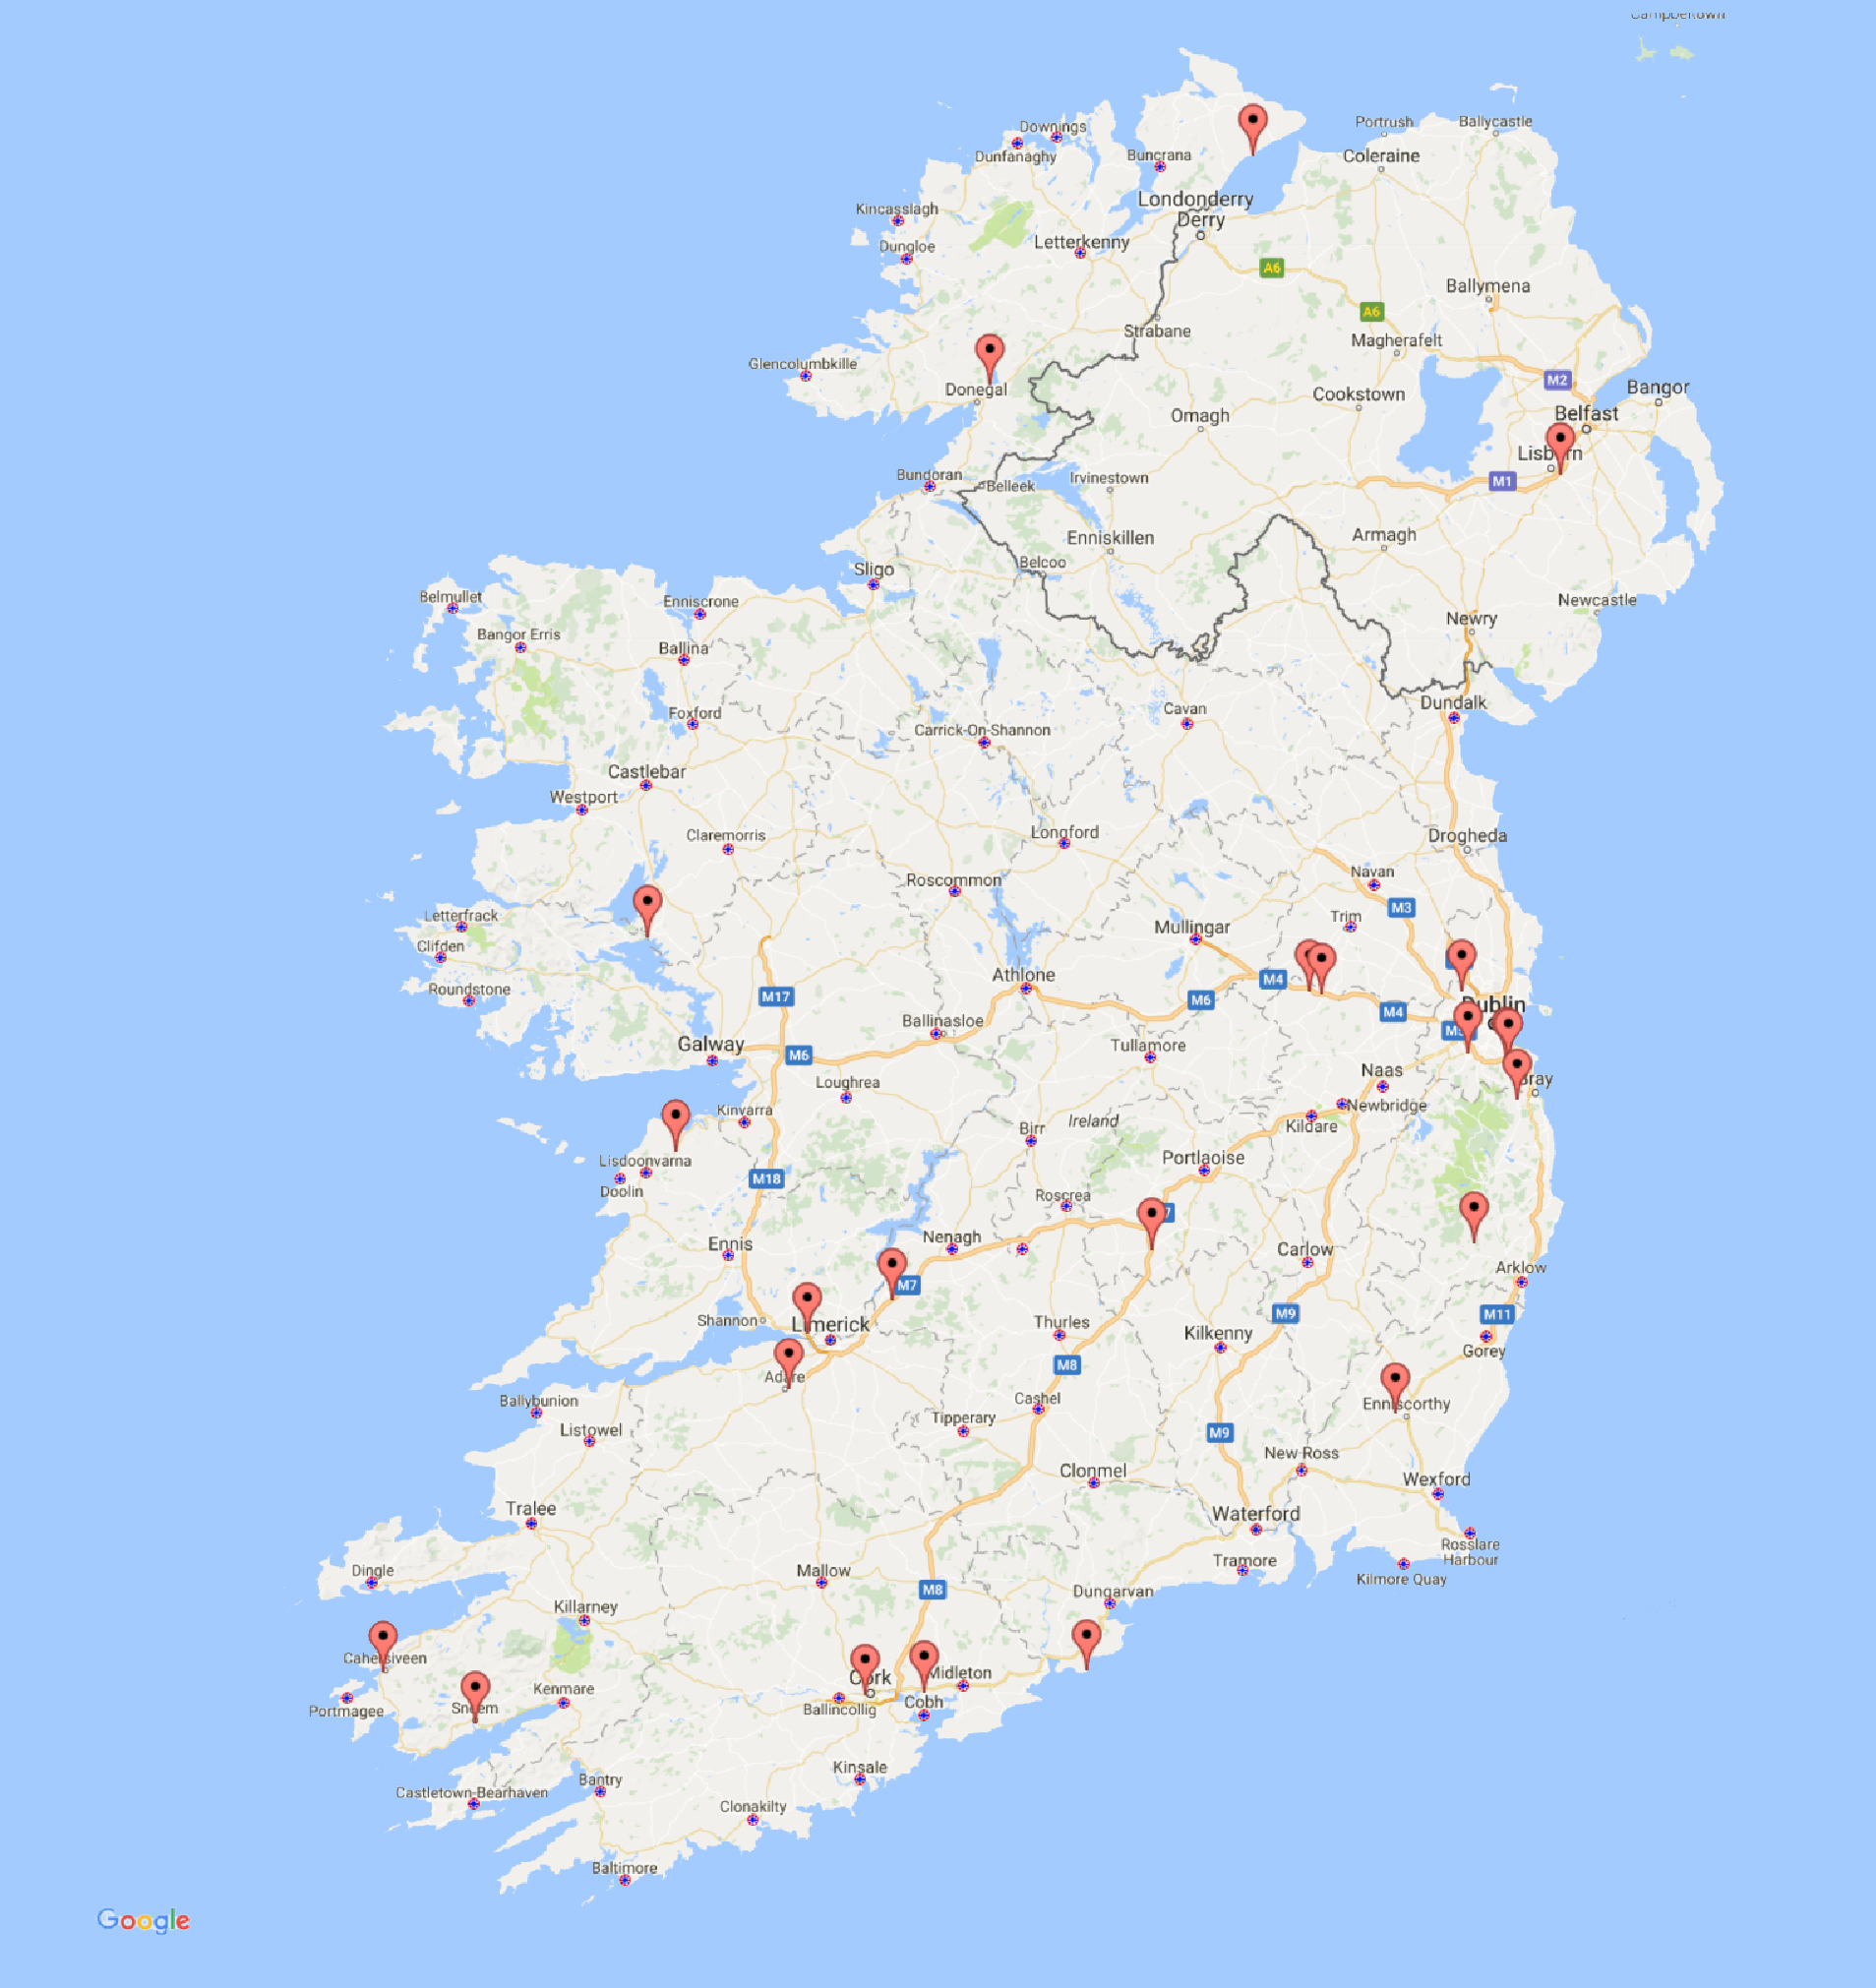
\includegraphics[width=2in]{stage1.pdf}
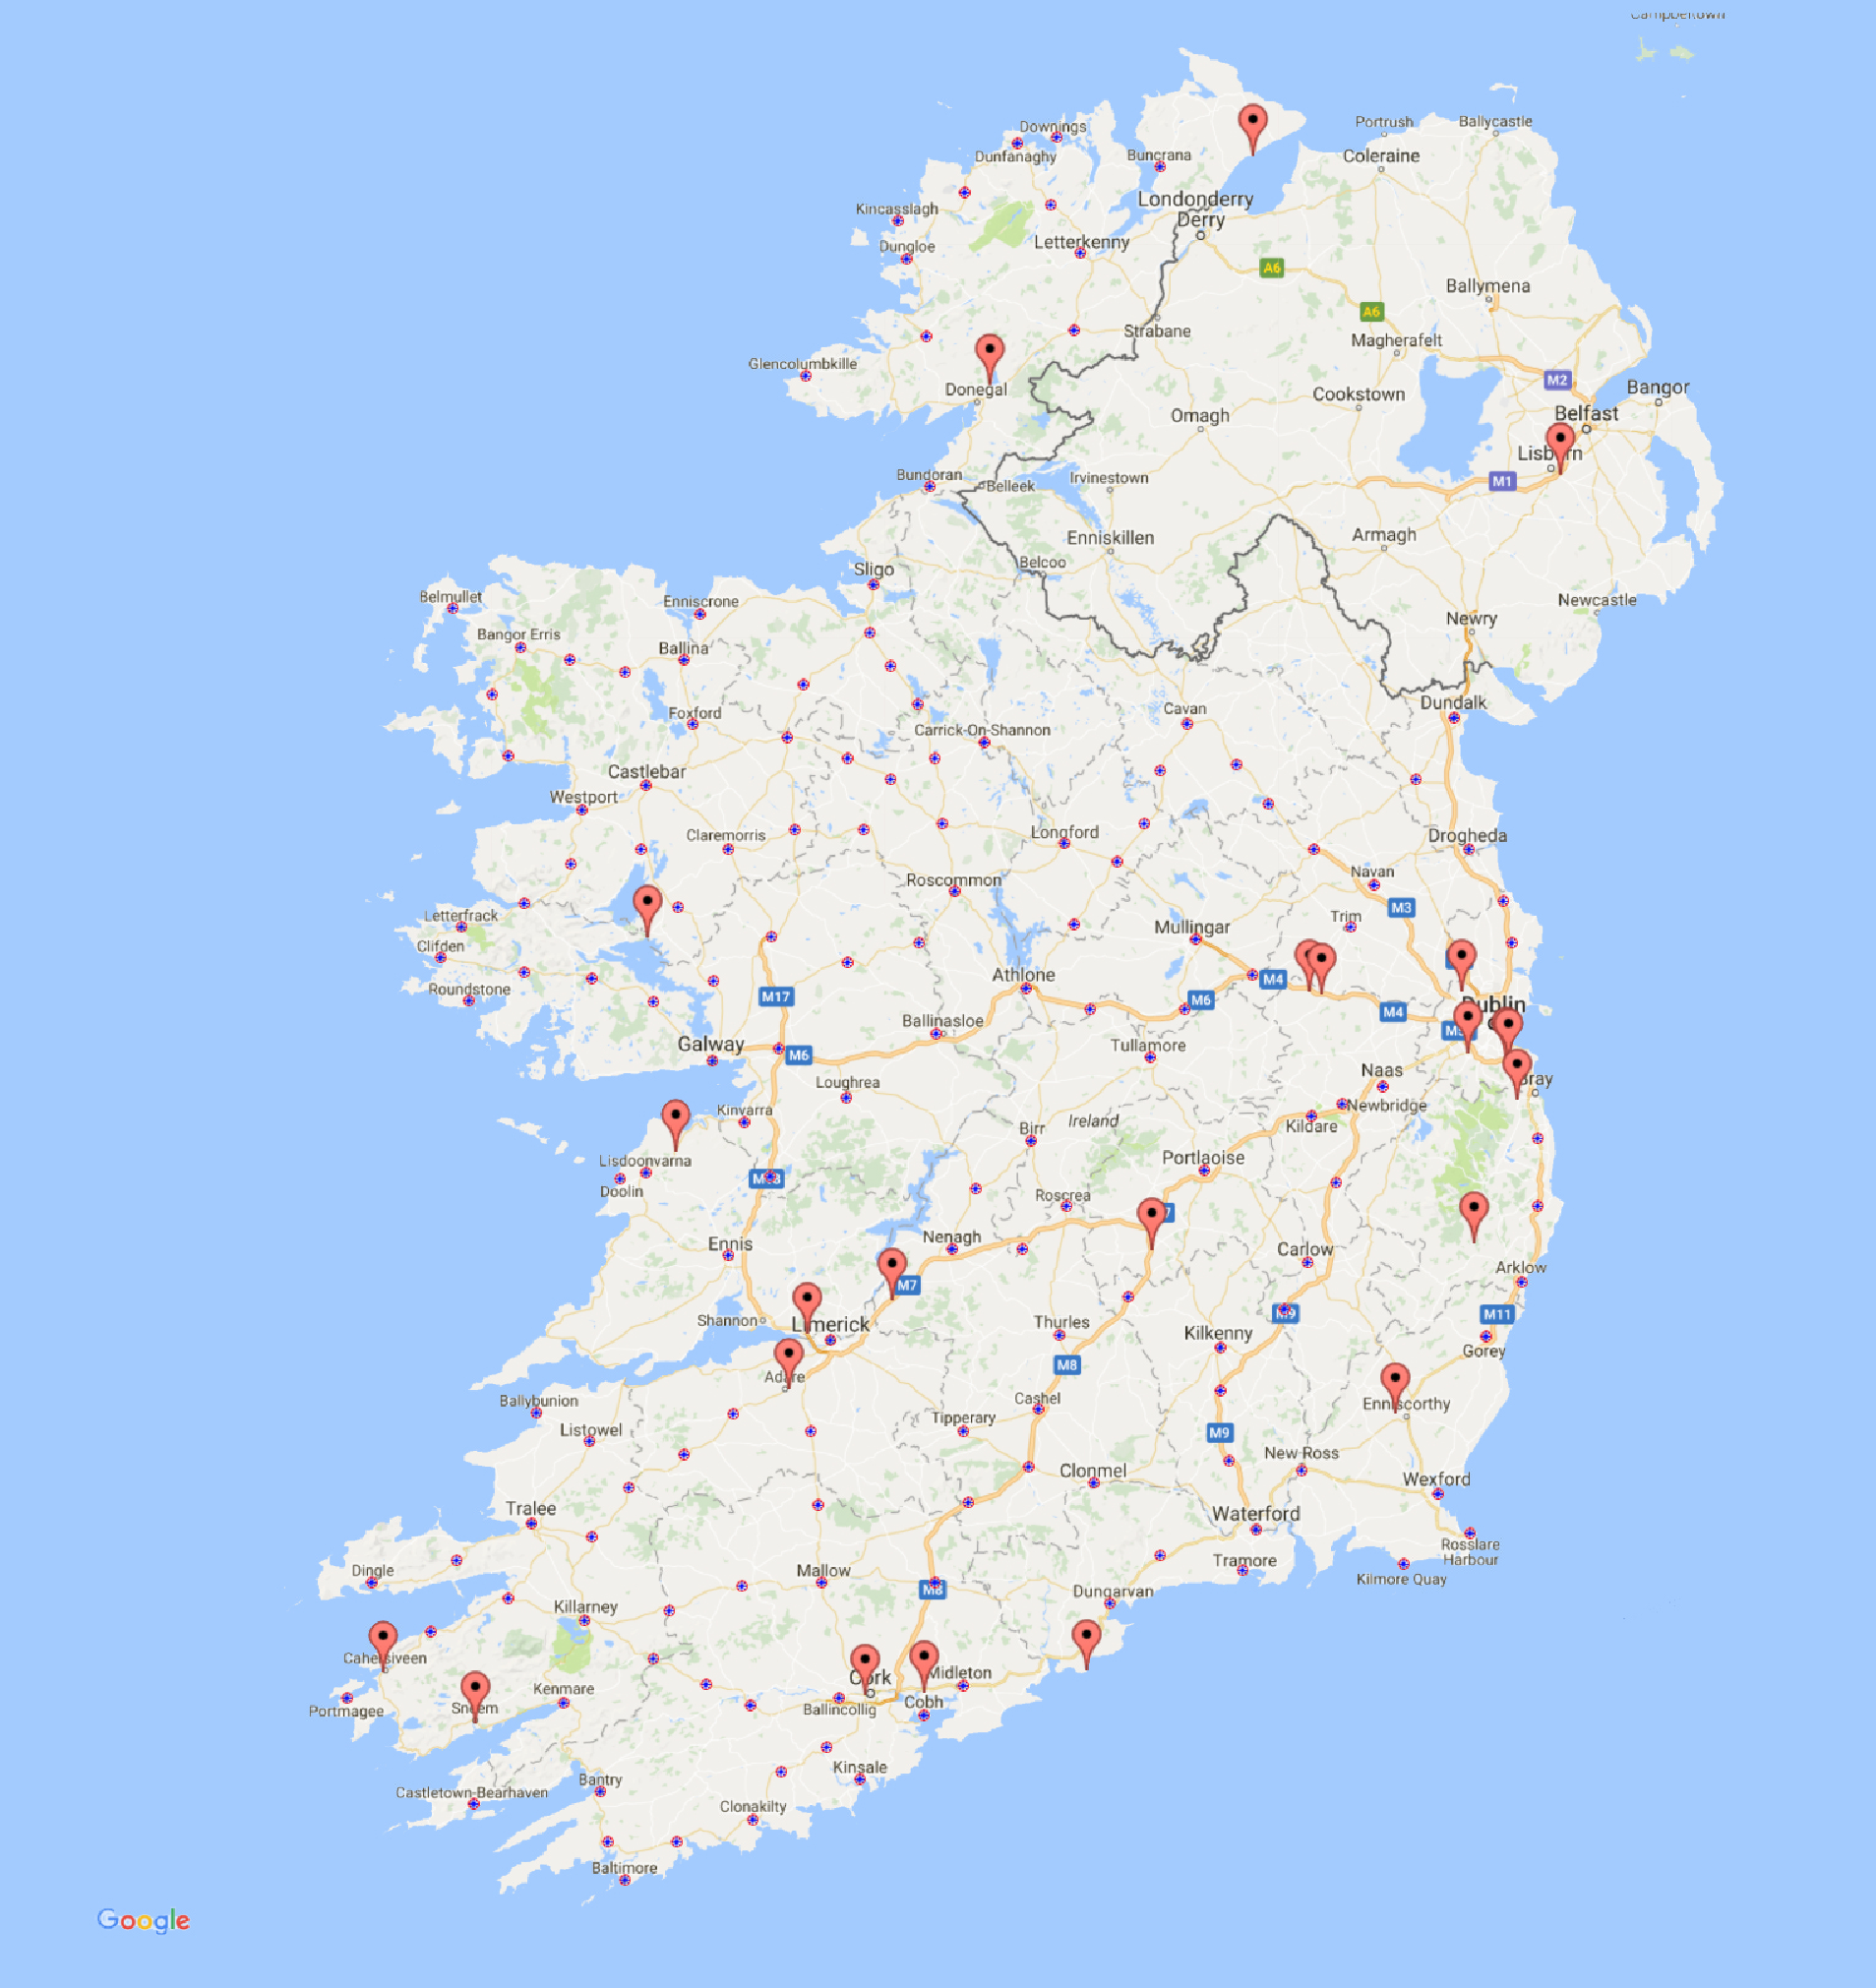
\includegraphics[width=2in]{stage2.pdf}
%\vspace{-0.1in}
\caption{Time evolution of the electric charging station in Ireland.}
\label{fig_stages}
%\vspace{-0.2in}
\end{figure}

We can apply this algorithm to find an optimal solution.
Based on the idea of Greedy Algorithm,
in every iteration,
the algorithm selects nodes in the subgraph induced by $X$ that will not disconnect the subgraph if we delete them from the subgraph.
Then we try to deselect the node with the highest cost $c_j, j \in N_{temp}$.
If $X^{'}$ meets the constrains in Problem~\ref{pro_optimal},
this algorithm shows that $X^{'}$ is a feasible solution.
Then, it continues to the next iteration.
Otherwise, it removes $j$ from $N_{temp}$,
then it deselect the node with the next highest cost.
The iterations terminate when $N_{temp}$ does not contain any node.
Finally, the output $X$ should be the optimal algorithm.

We apply this algorithm to the target nation (Ireland) 
,and try to find the optimal solution in different rates of electric vehicles.
Figure~\ref{fig_stages} shows the result of it.
We will discuss it later in next Section.
